%%%%%%%%%%%%%%%%%%%%%%%%%%%%%%%%%%%%%%%%%%%%%%%%%%%%%%%%%%%%%%%%%
%
% Project     : Bachelorarbeit
% Title       : Machbarkeitsanalyse für eine ressourcenorientierte Schnittstelle zur Verarbeitung grundlegender Probleme der Informatik
% File        : probleme.tex Rev. 01
% Date        : 01.03.2015
% Author      : Raffael Santschi
%
%%%%%%%%%%%%%%%%%%%%%%%%%%%%%%%%%%%%%%%%%%%%%%%%%%%%%%%%%%%%%%%%%

\chapter{Analyse und Auswahl der Probleme \resultAssignment{[R1]}}\label{chap.problemauswahl}
In diesem Kapitel werden die verschiedene Probleme, welche für die Erstellung der Schnittstelle betrachtet wurden, und das dazugehörige Auswahlverfahren erläutert.

\section{Auswahlverfahren}\label{cat_theo_inf}
Da es viele Probleme mit hoher Laufzeitkomplexität gibt, musste ein geeignetes Auswahlverfahren gefunden werden. Mit diesem Verfahren sollten möglichst unterschiedliche 
Typen dieser Probleme für die Schnittstelle evaluiert werden. Dafür wurde eine Kategorisierung der Probleme gesucht, auf welche sich gestützt werden konnte. In der Informatik wird oft 
das Buch "`Computers and Intractability: A Guide to the Theory of NP-Completeness"' \cite{garey1979computers} von Micheal Garey und David S. Johnson als Quelle verwendet. Laut einer 
Auswertung über die freie, digitale Bibliothek "`CiteSeer"' war es das mit 4137 Referenzen im Jahre 2006 am häufigsten Zitierte Informatik Werk der Bibliothek \cite{citeseer_algo_buch}. In 
diesem Buch werden verschiedene \gls{np}-vollständige und \gls{np}-schwere Probleme vorgestellt und in Kategorien unterteilt. Diese Kategorien (siehe Auflistung unten) wurden auch benutzt, 
um die zu analysierenden Probleme auszuwählen.

\begin{itemize}
	\item Graphentheorie
	\item Netzwerk Design
	\item Sets und Partitionen
	\item Speicherung und Wiederherstellung
	\item Sequenzierung und Planung
	\item Mathematisches Programmieren
	\item Algebra und Zahlentheorie
	\item Spiele und Puzzles
	\item Logik
	\item Automaten und Sprachtheorie
	\item Programm Optimierung
	\item Sonstiges
	\item Offene Probleme
\end{itemize}

Im Rahmen dieser Arbeit konnten nicht alle Probleme aus dem Buch behandelt werden. Deshalb wurde eine Auswahl von fünf Problemen getroffen, welche in der Realität auftreten und nicht 
nur von rein wissenschaftlichem Interesse sind. Bei der Auswahl wurde darauf geachtet, dass die Probleme aus unterschiedlichen Kategorien kommen. Es wurden jedoch auch zwei aus der 
gleichen Kategorie ausgesucht, um zu analysieren wie sich diese im Gegensatz zu den anderen verhalten. 

Die Probleme werden im folgenden Abschnitt genauer erläutert und für die weiteren Schritte der Erstellung der Schnittstelle berücksichtigt. Durch dieses Vorgehen konnte eine 
hohe Diversität von Problemen sichergestellt werden, was bei der Erstellung der Anforderungen und des Konzepts hilfreich war.

\section{Problemauswahl}\label{problem_selection}

\subsection{Hierarchie der Reduktion}\label{hierarchy_reduction}
Wie bereits in \ref{np_complet} beschrieben, muss für den Beweis der \gls{np}-Vollständigkeit bzw. \gls{np}-Schwere ein bekanntes \gls{np}-schweres Problem auf das Bestehende in 
\gls{polynomialzeit} reduziert werden können. In \autoref{fig:hierarchy_reduction} ist die Hierarchie der Reduktion für die ausgewählten Probleme aufgezeigt.

\begin{figure}[h]
\centering 
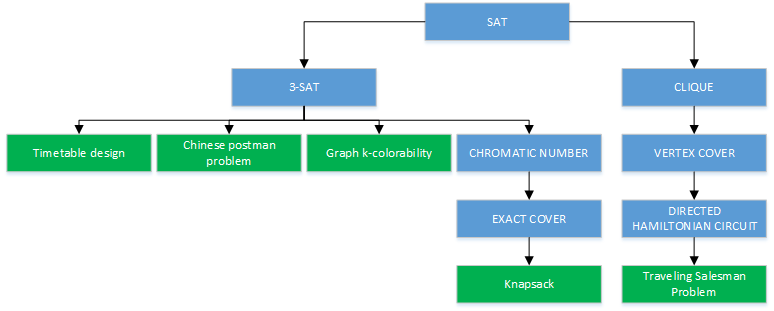
\includegraphics[scale=0.75]{images/visio/problem_hierarchy.png}
\caption[Hierarchie der Reduktion zum Beweis der NP-Vollständigkeit bzw. NP-Schwere]{Hierarchie der Reduktion zum Beweis der NP-Vollständigkeit bzw. NP-Schwere \selfmade{, Daten aus \cite{garey1979computers}}}
\label{fig:hierarchy_reduction}
\end{figure}

\subsection{Graphentheorie}\label{graph_theory}

	\subsubsection{Färbung (Graphtheorie)}\label{colarability_graph_theory}
	Die Färbung in der Graphtheorie ist ein \gls{np}-vollständiges Problem. Dies wurde durch die Reduktion des 3-SAT Problemes bewiesen.

	\paragraph{Beschreibung}
	Englischer Name: Graph k-colorability

	Bei diesem Problem geht es darum, die Knoten eines Graphens so zu färben, dass keine zwei benachbarten Knoten die gleiche Farbe tragen. Ein Graph heisst k-färbbar, wenn die 
Färbung mit k Farben korrekt durchgeführt werden kann. Dieses Problem ist für $k = 2$ in \glslink{polynomialzeit}{polynomieller} Zeit lösbar, für $k > 2$ jedoch nicht mehr. Es gibt Spezialfälle, 
bei welchen auch ein Problem mit $k > 2$ in \glslink{polynomialzeit}{polynomieller} Zeit lösbar sind (siehe \cite{garey1979computers}).

	\paragraph{Beispiel}
	Gegeben sei ein Graph mit 10 Knoten mit einer vorgegebenen Konfiguration (siehe \autoref{fig:graph_faerbung}).\\
	Gesucht ist die Färbung der Knoten, damit keine zwei benachbarten Knoten die gleiche Farbe haben. Zudem die minimale Anzahl Farben ($k$), welche verwendet werden müssen, damit 
	die Bedingung erfüllt ist. Der Graph \ref{fig:graph_faerbung_incorrect} zeigt eine ungültige Lösung mit zwei Farben. Es kann gezeigt werden, dass dieser Graph 
	mindestens drei Farben benötigt, um die Bedingung zu erfüllen (siehe Graph \ref{fig:graph_faerbung_correct}). Somit ist $k=3$.
\begin{figure}[ht]
\centering
\subfigure[Inkorrekte Färbung]{
  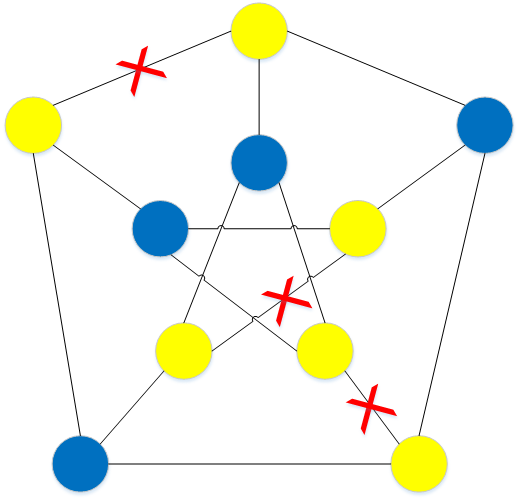
\includegraphics[scale=0.5]{images/visio/graph_faerbung_incorrect.png}
  \label{fig:graph_faerbung_incorrect}
}
\subfigure[Korrekte Färbung]{
  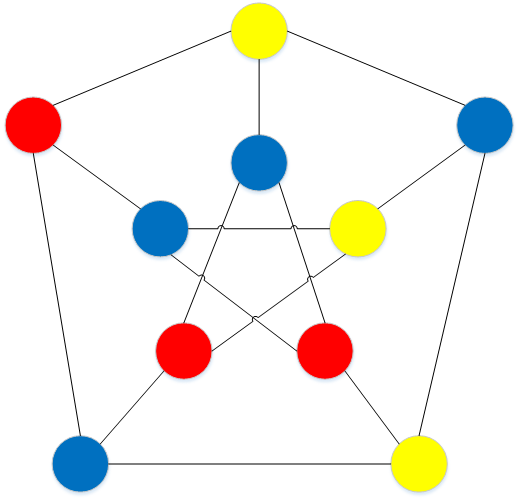
\includegraphics[scale=0.5]{images/visio/graph_faerbung_correct.png}
  \label{fig:graph_faerbung_correct}
}
\caption[Knotenfärbung eines Graphen mit 10 Knoten]{Kanten Färbung eines Graphen mit 10 Knoten \selfmade{}}
\label{fig:graph_faerbung}
\end{figure}

\FloatBarrier 
	\paragraph{Eingabe- und Ausgabedaten}\mbox{}\\
	Eingabedaten: Knoten und ihre Kanten\\
	Ausgabedaten: Knoten mit ihrer Färbung und $k$ (Anzahl benötigter Farben)

	\paragraph{Einfluss der Parameter auf die Komplexität}\mbox{}\\
	Bei der Knotenfärbung steigert sich die Komplexität mit Anzahl Kanten. Die Knoten sind nur insofern relevant, dass sie neue Kanten aufspannen. Dass die Komplexität nur von der Anzahl Kanten 
	abhängt, zeigt auch die Formel zur Berechnung des Maximums von $k$: $k \le \frac{1}{2} + \sqrt{2m + \frac{1}{4}}$, wobei $m$ für die Anzahl Kanten steht 
	(siehe \cite{seminar_rainer_graph}). Je grösser $k$, desto häufiger treten Kollisionen auf und umso mehr Varianten müssen ausprobiert werden.

	\paragraph{Bekannte Algorithmen}
	(siehe \cite{seminar_algo_graph}, \cite{krumke2012graphentheoretische} und \cite{seminar_rob_graphen})
	\begin{itemize}
		\item Spalten-Generierungs-Ansatz
		\item Sequentielles Färben (Sequential Coloring)
		\item Backtracking Algorithmus
		\item Greedy Algorithmus
		\item Johnson-Algorithmus
	\end{itemize}	

	\paragraph{Bekannte reale Probleme}	
	Es gibt einige reale Probleme, welche mit der Knotenfärbung gelöst werden können, hier eine Auswahl:
	\begin{itemize}
		\item Stundenplan: Anhand der eingegebenen Daten wird ein Konfliktmatrix erstellt und diese dann in ein Färbungsproblem umgewandelt. Die Anzahl benötigten Farben sind dann 
			die Anzahl der verschiedenen Perioden, welche es benötigt, um eine Stundenplan ohne Konflikte zu erstellen. \cite{ieee_exam_table_graph_coloring} \cite{time_table_graph_coloring} \cite{timetabling_abdullah}
		\item Frequenzverteilung (Mobilfunk): Im Mobilfunk hat jede Antenne einen Frequenzbereich. Im Graph werden die Antennen miteinander verbunden, bei denen sich die 
			Reichweite überschneidet. Die Farben können durch Frequenzen ersetzt werden. Die Lösung stellt eine konfliktfreie Mobilnetzabdeckung dar. \cite{seminar_rob_graphen}
		\item Einfärben von Landkarten: Die Länder sind die Knoten, die Kanten die Verbindung zu den Nachbarländern und die errechnete Farbe entspricht der Einfärbung auf der 
			Landkarte. \cite{seminar_rob_graphen}
	\end{itemize}

\newpage
\subsection{Netzwerk Design}\label{network_design}

	\subsubsection{Problem des Handlungsreisenden}\label{tsp}
	Das Problem des Handlungsreisenden ist ein \gls{np}-schweres Problem. Dies wurde durch die Reduktion des Hamiltonkreisproblemes bewiesen. Das Problem wird fälschlicherweise oft als 
	\gls{np}-vollständig bezeichnet. Es ist jedoch noch kein \gls{polynomialzeit_verifizierer} bekannt, der in \gls{polynomialzeit} überprüfen kann, ob die errechnete Route das optimale Resultat 
	ist.

	\paragraph{Beschreibung}
	Englischer Name: Traveling Salesperson Problem\\
	Beim Problem des Handlungsreisenden geht es darum, mit einer optimalen Route von einem Ausgangspunkt verschiedene Wegpunkte genau ein Mal abzufahren und wieder zum 
	Ausgangspunkt zurück zu kehren. Bei zehn Wegpunkten und gerichteten Kanten sind das über dreieinhalb Millionen Möglichkeiten. Bei der symmetrischen Variante mit ungerichteten Kanten 
	sind die Verbindungen zwischen zwei Punkten gleich lang, was die Komplexität halbiert. 

	\paragraph{Beispiel} Gegeben seien vier Wegpunkte (A, B, C, D), der Startpunkt sei A.\\
	Gesucht ist die optimale Route, welche alle Wegpunkte beinhaltet und wieder bei A endet.\\
	Die Abbildung \ref{fig:tsp_example} zeigt alle möglichen Lösungen mit ihren errechneten Werten. Die Route A-D-C-B-A ist mit Kosten von 16 die beste Route. Weiter ist zu sehen, 
	dass bei vier Wegpunkten mit gerichteten Kanten bereits sechs Möglichkeiten vorhanden sind.
\begin{figure}[h]
\centering
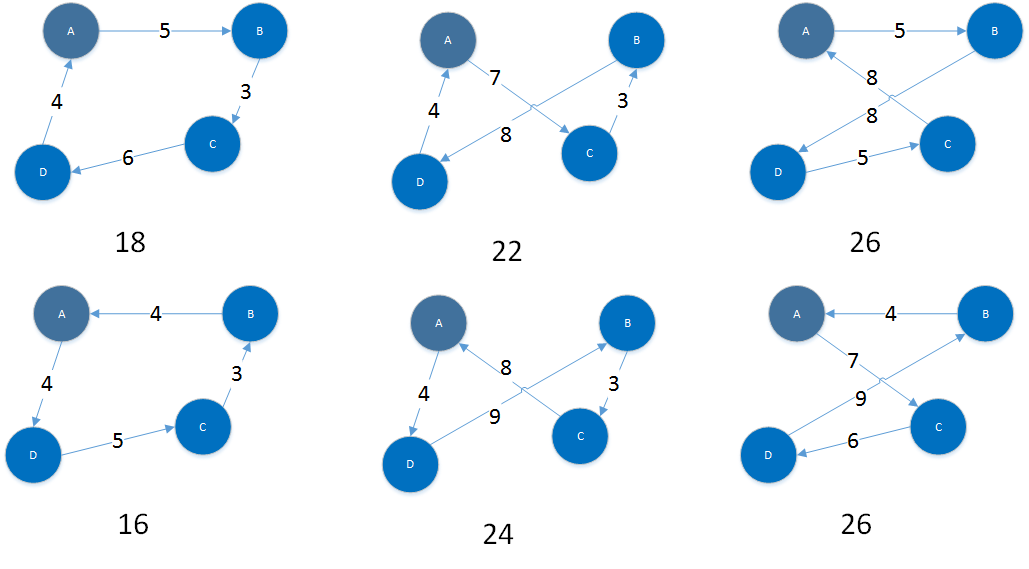
\includegraphics[scale=0.55]{images/visio/tsp.png}
\caption[Problem des Handlungsreisenden mit 4 Wegpunkten]{Problem des Handlungsreisenden mit vier Wegpunkten \selfmade{}}
\label{fig:tsp_example}
\end{figure}

	\paragraph{Eingabe- und Ausgabedaten}\mbox{}\\
	Eingabedaten: Startpunkt und Wegpunkte, welche passiert werden müssen\\
	Ausgabedaten: Reihenfolge der Wegpunkte für eine optimale Route

	\paragraph{Einfluss der Parameter auf die Komplexität}\mbox{}\\
	Die Komplexität beim Problem des Handlungsreisenden wird durch die Anzahl Wegpunkte bestimmt. Für die asymmetrische Variante ist die Formel zur Berechnung der Möglichkeiten $(n-1)!$ 
	für ein symmetrische hingegen $\frac{(n-1)!}{2}$.
	
	 \newpage
	\paragraph{Bekannte Algorithmen}\cite{tsp_algorithmen} \cite{tsp_semesterarbeit} \cite{pomberger2008algorithmen}
	\begin{itemize}
		\item Branch and Bound
		\item Nearest-Neighbor
		\item Christofides
	\end{itemize}

	\subsubsection{Briefträgerproblem}\label{chinese_postman}
	Das Briefträgerproblem ist an sich kein \gls{np}-vollständiges Problem, jedoch wurde für Varianten des Problems die \gls{np}-Vollständigkeit bewiesen. Für das `Rural Postman Problem`, 
	bei welchem nicht jeder Punkt zwingend abgefahren werden muss, wurde dies durch die Reduktion des 3-SAT Problemes bewiesen. In dieser Arbeit wird das Briefträgerproblem behandelt,
	da die Varianten darauf aufbauen und so die Basis betrachtet wird.

	\paragraph{Beschreibung}
	Englischer Name: Chinese postman problem\\
	Das Briefträgerproblem ist vergleichbar mit dem Problem des Handlungsreisenden, jedoch geht es darum jede Kante mindestens ein Mal abzufahren. Die Knoten stellen Kreuzungen dar, 
	die Kanten entsprechen den Strassen, beide dürfen mehrfach befahren werden. Die minimale Länge kann mit Hilfe des \glslink{eulerkreis}{Eulerkreises} relativ einfach berechnet werden. 
	Falls der Graph die Kriterien des \glslink{eulerkreis}{Eulerkreises} nicht erfüllt, werden alle Knoten mit ungerader Anzahl Kanten mit einem anderen Knoten verbunden. Für die Auswahl der 
	zu verbindenden Knoten wird die perfekte Paarung berechnet. Die minimal Länge ist die Summe aller Strecken und Hilfsstrecken. \cite{pearson2004decision}

	\paragraph{Beispiel} Gegeben sei der Graph mit den Punkten A bis H und den Verbindungen in blau.\\
Gesucht ist eine Route mit dem kürzesten Weg, welche jede Kante mindestens ein Mal abfährt. \cite{pearson2004decision}\\
Die grün eingezeichneten Verbindungen sind Hilfslinien, um den Graphen in einen \gls{eulerkreis} zu verwandeln. Eine mögliche Lösung mit der minimal Länge von 1000 ist die 
Route A-D-C-G-H-C-A-B-D-F-B-E-F-H-F-B-A.
\begin{figure}[h]
\centering
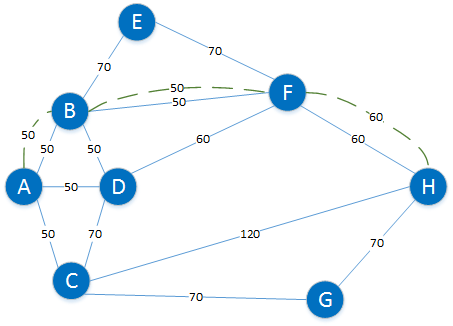
\includegraphics[scale=0.8]{images/visio/chinese_postman.png}
\caption[Beispiel für ein Briefträgerproblem]{Beispiel für ein Briefträgerproblem \selfmade{, Daten entnommen aus: \cite{pearson2004decision}}}
\label{fig:chinese_postman_example}
\end{figure}

	\paragraph{Eingabe- und Ausgabedaten}\mbox{}\\
	Eingabedaten: Startpunkt und Knoten mit ihren Verbindungen mit einer Gewichtung\\
	Ausgabedaten: Reihenfolge der Knoten für eine minimale Strecke

	\paragraph{Einfluss der Parameter auf die Komplexität}\mbox{}\\
	Wie bei der Knotenfärbung spielt die Anzahl Kanten die Hauptrolle bei der Komplexität. Wie viele Knoten ein Graph hat und ob dieser bereits \glslink{eulerkreis}{eulersch} ist, hat einen 
	geringeren Einfluss.

	\paragraph{Bekannte Algorithmen}\mbox{}\\
	Briefträgeralgorithmus (Chinese postman algorithm) \cite{pearson2004decision}

\subsection{Sequenzierung und Planung}\label{sequencing_scheduling}

	\subsubsection{Stundenplan-Erstellung}\label{tsp}
	Das Erstellen eines Stundenplans ist ein \gls{np}-vollständiges Problem. Dies wurde durch die Reduktion des 3-SAT-Problems bewiesen.

	\paragraph{Beschreibung}
	Englischer Name: Timetable design\\
	Die Erstellung von Stundenplänen ist ein sehr komplexes Problem. Basierend auf Fächer, Lehrer, Klassen und Klassenzimmern wird versucht, eine optimale Verteilung der Stunden zu 
	erreichen. Die wichtigste Bedingung ist, dass eine Ressource, sei das ein Lehrer, eine Klasse oder ein Schulzimmer, zu jedem Zeitpunkt höchstens ein Mal verplant ist. 
	Zusätzlich kann es beliebige weitere Kriterien geben, beispielsweise dass eine Klasse nie mehr als neun Lektionen pro Tag haben soll oder ein Lehrer nie mehr als 
	fünf Lektionen nacheinander unterrichten sollte. Bei der Erstellung von Stundenplänen wird oft von Hard Constraints und Soft Constraints gesprochen. Ein Hard Constraint ist im Gegensatz zu 
	einem Soft Constraint unabdingbar. Es ist nicht möglich, dass ein Lehrer zwei verschiedene Fächer gleichzeitig unterrichtet, notfalls könnte er aber mehr als fünf Lektionen hintereinander 
	unterrichten. \cite{Abramson92aparallel} \cite{Abramson91constructingschool} \cite{framework_timetabling} \cite{time_table_constraint_opti_ea}

	\paragraph{Beispiel} Gegeben seien die Fächer, Lehrer, Klassen und Klassenzimmer aus den Tabellen \ref{table:eg_subject}, \ref{table:eg_teacher}, \ref{table:eg_schoolclasses} und \ref{table:eg_schoolroom}.\\
Gesucht ist ein Stundenplan, bei welchem es keine Kollisionen für Lehrer, Klassen und Klassenzimmer gibt.

\begin{table}[ht]
\centering
  \begin{tabular}{ l | l }
	\hline
	\rowcolor{gray}
	\textbf{Fachname}	& \textbf{Kürzel}\\ \hline
	Mathematik		& M\\ \hline
	Deutsch		& D\\ \hline
	Englisch		& E\\ \hline
	Französisch		& F\\ \hline
	Sport			& Sp
  \end{tabular}
   \caption{Schulfächer}\label{table:eg_subject}
\end{table}

\begin{table}[ht]
\centering
  \begin{tabular}{ l | l }
	\hline
	\rowcolor{gray}
	\textbf{Lehrername} 	& \textbf{Ausbildung}\\ \hline
	Angst				& Deutsch, Mathematik, Sport\\ \hline
	Arm				& Sport\\ \hline
	Bernasconi			& Deutsch, Mathematik, Französisch\\ \hline
	Müller				& Deutsch, Mathematik, Englisch, Französisch\\ \hline
	Pfister				& Englisch, Französisch
  \end{tabular}
   \caption{Lehrer}\label{table:eg_teacher}
\end{table}

\begin{table}[ht]
\centering
  \begin{tabular}{ l | l }
	\hline
	\rowcolor{gray}
	\textbf{Klassenname} 	& \textbf{Benötigte Fächer}\\ \hline
	Tja13				& Deutsch, Mathematik, Sport\\ \hline
	Tja12				& Deutsch, Mathematik, Sport, Französisch\\ \hline
	Tja11				& Deutsch, Mathematik, Sport, Französisch, Englisch\\ \hline
	Tja10				& Deutsch, Mathematik, Sport, Französisch, Englisch
  \end{tabular}
   \caption{Klassen}\label{table:eg_schoolclasses}
\end{table}

\begin{table}[ht]
\centering
  \begin{tabular}{ l }
	\hline
	\rowcolor{gray}
	\textbf{Zimmername}\\ \hline
	Zimmer 101\\ \hline
	Zimmer 103\\ \hline
	Zimmer 201\\ \hline
	Turnhalle
  \end{tabular}
   \caption{Klassenzimmer}\label{table:eg_schoolroom}
\end{table}

\FloatBarrier
\autoref{table:timetable_1} zeigt eine mögliche Lösung. Es wurde beachtet, dass die Lehrer möglichst gleich viele Stunden unterrichten und die Schüler keine doppelten Freistunden haben. Es 
fällt auf, dass das Zimmer 201 nur selten besetzt ist. In der zweiten Variante (siehe \autoref{table:timetable_2}) wurden die Stunden der Klasse Tja11 so verschoben, dass 
das Zimmer 201 gar nicht mehr benötigt wird. Die Klasse Tja11 hat nun aber eine doppelte Freistunde. Die Eingabedaten sind im Beispiel noch sehr überschaubar, 
trotzdem gibt es bereits enorm viele verschiedenen Möglichkeiten und Ausprägungen.

\begin{table}[ht]
\centering
  \begin{tabular}{ l | l | l | l | l }
	\hline
	\rowcolor{gray}
	\textbf{Uhrzeit} 	& \textbf{Turnhalle}	& \textbf{Zimmer 101} 	& \textbf{Zimmer 103}	&  \textbf{Zimmer 201}\\ \hline
	0800-0900		& Sp / Tja13 / Arm		& D / Tja11 / Müller		& 				& \\ \hline
	0900-1000		& Sp / Tja13 / Arm		& M / Tja11 / Müller		& F / Tja12 / Pfister		& \\ \hline
	1000-1100		& Sp / Tja12 / Arm		& D / Tja10 / Bernasconi	& M / Tja13 / Angst		& F / Tja11 / Müller\\ \hline
	1100-1200		& Sp / Tja12 / Arm		& M / Tja10 / Angst		& D / Tja13 / Bernasconi	& E / Tja11 / Pfister\\ \hline \hline
	1300-1400		& Sp / Tja11 / Angst	& F / Tja10 / Bernasconi	& D / Tja12 / Müller		& \\ \hline
	1400-1500		& Sp / Tja11 / Angst	& E / Tja10 / Pfister		& M / Tja12 / Bernasconi	& \\ \hline
	1500-1600		& Sp / Tja10 / Angst	& 				& 				& \\ \hline
	1600-1700		& Sp / Tja10 / Angst	& 				& 				& \\ \hline
  \end{tabular}
   \caption{Möglicher Stundenplan - Variante 1}\label{table:timetable_1}
\end{table}

\begin{table}[ht]
\centering
  \begin{tabular}{ l | l | l | l }
	\hline
	\rowcolor{gray}
	\textbf{Uhrzeit} 	& \textbf{Turnhalle}	& \textbf{Zimmer 101} 	& \textbf{Zimmer 103}	\\ \hline
	0800-0900		& Sp / Tja13 / Arm		& D / Tja11 / Müller		& 				\\ \hline
	0900-1000		& Sp / Tja13 / Arm		& M / Tja11 / Müller		& F / Tja12 / Pfister		\\ \hline
	1000-1100		& Sp / Tja12 / Arm		& D / Tja10 / Bernasconi	& M / Tja13 / Angst		\\ \hline
	1100-1200		& Sp / Tja12 / Arm		& M / Tja10 / Angst		& D / Tja13 / Bernasconi	\\ \hline \hline
	1300-1400		& Sp / Tja11 / Angst	& F / Tja10 / Bernasconi	& D / Tja12 / Müller		\\ \hline
	1400-1500		& Sp / Tja11 / Angst	& E / Tja10 / Pfister		& M / Tja12 / Bernasconi	\\ \hline
	1500-1600		& Sp / Tja10 / Angst	& F / Tja11 / Müller		& 				\\ \hline
	1600-1700		& Sp / Tja10 / Angst	& E / Tja11 / Pfister		& 				\\ \hline
  \end{tabular}
   \caption{Möglicher Stundenplan - Variante 2}\label{table:timetable_2}
\end{table}

\FloatBarrier

	\paragraph{Eingabe- und Ausgabedaten}\mbox{}\\
	Eingabedaten: Fächer, Lehrer, Klassen und Klassenzimmer mit verschiedenen Einschränkungen und Zusatzinformationen\\
	Ausgabedaten: Einteilung der Fächer mit den dazugehörigen Klassen, Lehrern und Zimmer auf verschiedene Tage und Uhrzeiten, welche keine Konflikte enthält

	\paragraph{Einfluss der Parameter auf die Komplexität}\mbox{}\\
	Beim Stundenplanproblem sind es nicht alle vier Listen, welche die Komplexität des Problems ausmachen. Den grössten Einfluss haben die Anzahl Stunden, welche verplant werden 
	müssen. Die Anzahl Möglichkeiten berechnen sich wie folgt (vergleiche \cite{scheduling_komplex}): 
	\[(Anzahl Räume * Anzahl Zeitfenster * Anzahl Lehrer)^{Anzahl Veranstaltungen}\]

	\paragraph{Bekannte Algorithmen}
	(siehe \cite{framework_timetabling})
	\begin{itemize}
		\item Backtracking Algorithmus
		\item Evolutionäre Algorithmen
		\item Constraint Logic Programming
	\end{itemize}	

	\paragraph{Bekannte ähnliche Probleme}	
	Es gibt diverse andere Planungsprobleme, welche auf dem gleichen Konzept basieren, jedoch unterschiedliche Eingabedaten und Beschränkungen haben \cite{framework_timetabling}:
	\begin{itemize}
		\item Spielplan
		\item Prüfungsplan
		\item Schichtenplanung
	\end{itemize}

	\paragraph{Bekannte Lösungen}		
	Eine gut ausgearbeitete Software ist 'Units' \cite{unit_express}, sie liefert umfangreiche Funktionen zur Erstellung von Stundenplänen.

\subsection{Mathematisches Programmieren}\label{mathematical_programming}

	\subsubsection{Rucksack-Problem}\label{knapsack}
	Das Rucksack-Problem ist ein \gls{np}-schweres Problem. Dies wurde durch die Reduktion des Problems der exakten Überdeckung bewiesen. Das Problem wird fälschlicherweise oft als 
	\gls{np}-vollständig bezeichnet. Es ist jedoch noch kein \gls{polynomialzeit_verifizierer} bekannt, der in \gls{polynomialzeit} überprüfen kann, ob die errechnete Lösung das optimale Resultat 
	ist.

	\paragraph{Beschreibung}
	Englischer Name: Knapsack\\
	Beim Rucksack-Problem geht es um einen beliebigen Behälter, symbolisch der Rucksack, mit einer Gewichtsschranke. Zudem gibt es Objekte, welche in den Container gepackt werden 
	können. Diese Objekte besitzen ein Gewicht und einen Profit. Das Ziel ist es, den grösstmöglichen Profit zu erlangen, ohne die Gewichtsschranke zu überschreiten. 
	\cite{knapsack_desc_web}

	\paragraph{Beispiel} Gegeben sei ein Rakete mit der Gewichtsschranke 645 kg und die Objekte in Tabelle \ref{table:knapsack_objects}.\\
Gesucht ist die Objektauswahl mit dem grössten Profit, welche die Gewichtsschranke nicht überschreitet.\\
In diesem Beispiel wäre die optimale Lösung 1, 2, 3 und 5. \cite{knapsack_desc_web}

\begin{table}[ht]
\centering
  \begin{tabular}{ c | r | r }
	\hline
	\rowcolor{gray}
	\textbf{Objekt-Nr.}	&	\textbf{Gewicht in kg}	&	\textbf{Profit}\\ \hline
	1			&	153			&	232\\ \hline
	2			&	54			&	73\\ \hline
	3			&	191			&	201\\ \hline
	4			&	66			&	50\\ \hline
	5			&	239			&	141\\ \hline
	6			&	137			&	79\\ \hline
	7			&	148			&	48\\ \hline
	8			&	249			&	38
  \end{tabular}
   \caption[Knapsack Objekte mit Gewicht und Profit]{Knapsack Objekte mit Gewicht und Profit (Daten aus \cite{knapsack_desc_web})}\label{table:knapsack_objects}
\end{table}

	\paragraph{Eingabe- und Ausgabedaten}\mbox{}\\
	Eingabedaten: Gewichtsschranke und Elemente mit Gewicht und Nutzwert\\
	Ausgabedaten: Zusammenstellung der Elemente mit dem höchsten Nutzwert

	\paragraph{Einfluss der Parameter auf die Komplexität}\mbox{}\\
	Die Komplexität des Rucksack-Problems hängt von der Anzahl der Objekte ab, die Gewichtsschranke trägt nicht zur Komplexität bei.

	\paragraph{Bekannte Algorithmen}
	\begin{itemize}
		\item Backtracking Algorithmus
		\item Greedy Algorithmus
		\item Algorithmus von Nemhauser und Ullmann \cite{knapsack_desc_web}
	\end{itemize}	

	\paragraph{Bekannte reale Probleme}
	Es gibt einige reale Probleme, welche mit der Rucksack-Problem gelöst werden können \cite{kellerer2004knapsack}, hier eine Auswahl:	
	\begin{itemize}
		\item Ausschneiden von verschiedenen Stücken aus einer Metall- oder Holzplatte: Optimale Nutzung der Fläche(n), damit am Schluss genug Einzelstücke für das Herstellen 
			des Endproduktes vorhanden sind.
		\item Kreditvergabe: Optimale Ausnutzung des Kreditbudgets mit der Vergabe von Krediten an Kunden, welche einen Kredit über eine gewisse Höhe haben möchten und eine 
			bestimmte Risikoeinstufung aufweisen.
	\end{itemize}


\newpage
\subsection{Logik}\label{logic}
Die in diesem Abschnitt aufgeführten Probleme sind der Vollständigkeit halber aufgelistet und beschrieben. Sie werden nicht für die weiteren Schritte der Schnittstelle verwendet, bilden jedoch 
die Grundpfeiler der \gls{np}-Vollständigkeit. Auf diese Grundpfeiler basieren zahlreiche Beweise der \gls{np}-Vollständigkeit von Problemen.

	\subsubsection{Erfüllbarkeitsproblems der Aussagenlogik (SAT)}\label{sat}
	Das Erfüllbarkeitsproblem der \gls{aussagenlogik} ist ein \gls{np}-vollständiges Problem. Dies wurde durch Stephen A. Cook in den 1970er Jahren bewiesen \cite{cook_complexity}.

	\paragraph{Beschreibung}
	Englischer Name: Satisfiability (SAT)\\
	Beim Erfüllbarkeitsproblem der \gls{aussagenlogik} ist zu überprüfen, ob eine beliebige \glslink{aussagenlogik}{aussagenlogische} Formel erfüllbar ist.	

	\paragraph{Beispiel} Gegeben sei eine \glslink{aussagenlogik}{aussagenlogische} Formel \ref{eq:aussagenlogik}.\\
	Gesucht ist die Antwort auf die Erfüllbarkeit dieser Formel.\\
	Die \autoref{table:sat_results} zeigt, dass die Formel für die Kombinationen 3, 4 und 8 erfüllbar ist.

	\begin{equation}
   		(A \vee B) \wedge C
  		 \label{eq:aussagenlogik}
	\end{equation}

\begin{table}[ht]
\centering
  \begin{tabular}{ c | c | c | c | c | c}
	\hline
	\rowcolor{gray}
	\textbf{Kombination-Nr.}	&	\textbf{A}	&	\textbf{B} 	& 	\textbf{C} 	&	$A \vee B$	&	\textbf{Resultat}\\ \hline
	1			&	wahr	& 	falsch	& 	falsch	&	wahr		&	falsch\\ \hline
	2			&	wahr	& 	wahr	& 	falsch	&	wahr		&	falsch\\ \hline
	\textbf{3}		&	wahr	& 	falsch	& 	wahr	&	wahr		&	\textbf{wahr}\\ \hline
	\textbf{4}		&	wahr	& 	wahr	& 	wahr	&	wahr		&	\textbf{wahr}\\ \hline
	5			&	falsch	& 	falsch	& 	falsch	&	falsch		&	falsch\\ \hline
	6			&	falsch	& 	wahr	& 	falsch	&	wahr		&	falsch\\ \hline
	7			&	falsch	& 	falsch	& 	wahr	&	falsch		&	falsch\\ \hline
	\textbf{8}		&	falsch	& 	wahr	& 	wahr	&	wahr		&	\textbf{wahr}\\ \hline
  \end{tabular}
   \caption{Wahrheitstabelle zur \glslink{aussagenlogik}{aussagenlogischen} Formel}\label{table:sat_results}
\end{table}

\newpage
	\subsubsection{3-SAT}\label{3sat}
	Das 3-SAT Problem ist ein \gls{np}-vollständiges Problem. Dies wurde durch die Reduktion des SAT Problems bewiesen.

	\paragraph{Beschreibung}
	Englischer Name: 3-Satisfiability (3-SAT)\\
	Das 3-SAT Problem ist eine Spezialfall des SAT Problems, es dürfen maximal 3 Literale in einer Klausel enthalten sein.

	\paragraph{Beispiel} Gegeben sei eine 3-SAT Formel \ref{eq:aussagenlogik_3sat}.\\
	Gesucht ist die Antwort auf die Erfüllbarkeit dieser Formel.\\
	Die \autoref{table:3sat_results} beweist, dass die Formel erfüllbar ist, lediglich für die Kombinationen 5, 11, 13 und 15 ist sie nicht korrekt.

	\begin{equation}
   		(A \wedge B \wedge C) \vee (B \wedge \neg C \wedge D)
  		 \label{eq:aussagenlogik_3sat}
	\end{equation}

\begin{table}[ht]
\centering
  \begin{tabular}{ c | c | c | c | c | c | c | c}
	\hline
	\rowcolor{gray}
	\textbf{Kombination-Nr.}	& \textbf{A}	& \textbf{B} 	& \textbf{C} & \textbf{D}  & $A \wedge B \wedge C$ & $B \wedge \neg C \wedge D$	& \textbf{Resultat}\\ \hline
	\textbf{1}			& wahr	& falsch	& falsch	& wahr	& wahr			 & wahr				& \textbf{wahr}\\ \hline
	\textbf{2}			& wahr	& wahr	& falsch	& wahr	& wahr			 & wahr 				& \textbf{wahr}\\ \hline
	\textbf{3}			& wahr	& falsch	& wahr	& wahr	& wahr			 & wahr				& \textbf{wahr}\\ \hline
	\textbf{4}			& wahr	& wahr	& wahr	& wahr	& wahr			 & wahr				& \textbf{wahr}\\ \hline
	5				& falsch	& falsch	& falsch	& wahr	& falsch			 & wahr				& falsch\\ \hline
	\textbf{6}			& falsch	& wahr	& falsch	& wahr	& wahr			 & wahr				& \textbf{wahr}\\ \hline
	\textbf{7}			& falsch	& falsch	& wahr	& wahr	& wahr			 & wahr 				& \textbf{wahr}\\ \hline
	\textbf{8}			& falsch	& wahr	& wahr	& wahr	& wahr			 & wahr 				& \textbf{wahr}\\ \hline
	\textbf{9}			& wahr	& falsch	& falsch	& falsch	& wahr			 & wahr				& \textbf{wahr}\\ \hline
	\textbf{10}			& wahr	& wahr	& falsch	& falsch	& wahr			 & wahr 				& \textbf{wahr}\\ \hline
	11				& wahr	& falsch	& wahr	& falsch	& wahr			 & falsch				& falsch\\ \hline
	\textbf{12}			& wahr	& wahr	& wahr	& falsch	& wahr			 & wahr				& \textbf{wahr}\\ \hline
	13				& falsch	& falsch	& falsch	& falsch	& falsch			 & wahr				& falsch\\ \hline
	\textbf{14}			& falsch	& wahr	& falsch	& falsch	& wahr			 & wahr				& \textbf{wahr}\\ \hline
	15				& falsch	& falsch	& wahr	& falsch	& wahr			 & falsch 				& falsch\\ \hline
	\textbf{16}			& falsch	& wahr	& wahr	& falsch	& wahr			 & wahr 				& \textbf{wahr}\\ \hline
  \end{tabular}
   \caption{Wahrheitstabelle zur 3-SAT Formel}\label{table:3sat_results}
\end{table}

\newpage
\section{Übersicht Eingabe- und Ausgabedaten \resultAssignment{[R2]}}\label{overview_input_output}
Die Eingabe- und Ausgabedaten der Probleme sind sehr unterschiedlich und weisen unterschiedliche Komplexität auf. Um einen besseren Überblick zu erhalten, wurden sie in der 
\autoref{table:input_output} zusammengefasst.
\begin{table}[ht]
\centering
  \begin{tabular}{ p{3cm} | p{5.4cm} | p{5.4cm} }
	\hline
	\rowcolor{gray}
	\textbf{Problem}				& \textbf{Eingabedaten}								& \textbf{Ausgabedaten}\\ \hline
	Färbung (Graphtheorie)			& \begin{enumerate}
								\item Knoten und ihre Kanten
							   \end{enumerate}				
							&  \begin{enumerate}
								\item Knoten mit ihrer Färbung
								\item $k$ (Anzahl benötigter Farben)
							   \end{enumerate}	\\ \hline
	Problem des Handlungsreisenden		& \begin{enumerate}
								\item Startpunkt
								\item Wegpunkte, welche passiert werden müssen
							   \end{enumerate}				
							&  \begin{enumerate}
								\item Wegpunkte in der Reihenfolge der optimalen Route
								\item Länge der Strecke
							   \end{enumerate}	\\ \hline
	Briefträgerproblem	 			& \begin{enumerate}
								\item Startpunkt
								\item Knoten mit ihren Verbindungen mit Gewichtung
							   \end{enumerate}				
							&  \begin{enumerate}
								\item Knoten in der Reihenfolge der minimalen Strecke
								\item Länge der Strecke
							   \end{enumerate}	\\ \hline
	Stundenplan-Erstellung			& \begin{enumerate}
								\item Fächer
								\item Lehrer
								\item Klassen
								\item Klassenzimmer
								\item Stundenplan Rahmenbedingungen
							   \end{enumerate}				
							&  \begin{enumerate}
								\item  Einteilung der Fächer mit den dazugehörigen Klassen, Lehrern und Zimmer auf verschiedene Tage und Uhrzeiten, welche keine 
									Konflikte enthält
							   \end{enumerate}	\\ \hline
	Rucksack-Problem				& \begin{enumerate}
								\item Gewichtsschranke
								\item Elemente mit Gewicht und Nutzwert
							   \end{enumerate}				
							&  \begin{enumerate}
								\item Zusammenstellung von den Elementen mit höchstem Nutzwert
								\item Nutzwert
							   \end{enumerate}	\\ \hline
  \end{tabular}
   \caption{Eingabe- und Ausgabedaten der ausgewählten Probleme}\label{table:input_output}
\end{table}

\newpage
\section{Beispiel für den Einfluss der Parameter auf die Komplexität \resultAssignment{[R1a]}}\label{example_complexity_knapsack}
Bei den vorgestellten Problemen wurde der Einfluss der Parameter auf die Komplexität der Probleme erwähnt. Um dies zu verdeutlichen wurde ein praktisches Beispiel anhand des 
Rucksack-Problems erstellt.

\subsection{Ausgangslage}
Das Rucksack-Problem hat zwei Eingabeparameter, zum einen die Gewichtsschranke und zum anderen die Elemente. Im Beispiel wurden verschiedene Anzahl Elemente verwendet und dies mit 
unterschiedlichen Gewichtsschranken kombiniert. Zum Vergleich wurde die Zeit gestoppt, welche der Brute Force-Algorithmus benötigt, um die optimale Lösung herauszufinden. Bei dieser 
Methode wird das Ergebnis zwar durch andere Prozesse auf dem Testsystem verfälscht, reicht jedoch für eine Veranschaulichung der Einflüsse.

\subsection{Resultat}
Die Berechnungszeiten waren ungenau und unterschiedlich. Das Resultat bestätigt jedoch bei jedem Versuch die Theorie, dass die Komplexität nur durch die Anzahl an Elementen 
beeinflusst wird. Die verschiedenen Berechnungszeiten wurden in der \autoref{table:example_complexity_knapsack} festgehalten. Mit einer höheren Gewichtsschranke bleibt die 
Berechnungszeit in etwa gleich, bei einer Erhöhung der Anzahl Elemente nimmt die Komplexität jedoch sehr schnell zu.

\begin{table}[ht]
\centering
  \begin{tabular}{ l | r | r | r | r | r }
	\hline
	\rowcolor{gray}
	\backslashbox{Gewichtsschranke:}{Anzahl an Elemente:}	& \textbf{10}	& \textbf{15} 	& \textbf{18}	& \textbf{20}	& \textbf{22}\\ \hline
	\textbf{10}							& 4ms			& 23ms		& 129ms		& 1079ms		& 7267ms 	\\ \hline
	\textbf{100}							& 1ms			& 16ms		& 149ms		& 1761ms		& 6054ms	\\ \hline
	\textbf{1000}						& 1ms			& 7ms			& 595ms		& 1038ms		& 6331ms	\\ \hline
	\textbf{10000}						& 1ms			& 7ms			& 48ms		& 583ms		& 7174ms	\\ \hline
  \end{tabular}
   \caption[Berechnungszeiten bei verschiedenen Eingabeparametern für das Rucksack-Problem]{Berechnungszeiten bei verschiedenen Eingabeparametern für das Rucksack-Problem}
   \label{table:example_complexity_knapsack}
\end{table}

In \autoref{fig:example_complexity_knapsack} wird die exponentielle Steigerung der Berechnungsdauer mit zunehmender Anzahl an Elementen sehr schön verdeutlicht.

\begin{figure}[h]
\centering
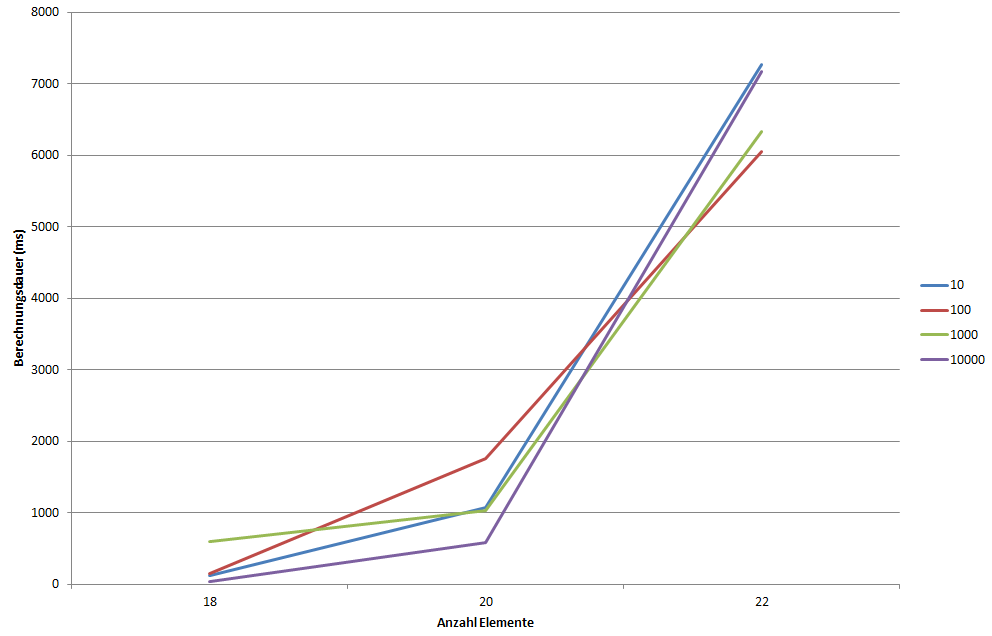
\includegraphics[scale=0.45]{images/excel/knapsack_complexity_example.png}
\caption[Berechnungszeiten für das Rucksack-Problem mit verschiedenen Eingabeparametern im Vergleich]{Berechnungszeiten für das Rucksack-Problem mit verschiedenen Eingabeparametern 
im Vergleich \selfmade{}}
\label{fig:example_complexity_knapsack}
\end{figure}
